\documentclass{article}
\usepackage[utf8]{inputenc}
% are all of these packages really necessary?
% no.
% i'm just too lazy to only grab the packages i want for a specific
% document, so i just glob all of my most commonly used packages together
% this is bad practice.
\usepackage{amsmath,amsthm,amssymb,amsfonts, fancyhdr, color, comment, graphicx, environ, mdframed, soul, calc, enumitem, mdframed, xcolor, geometry, empheq, mathtools, tikz, pgfplots, caption, subcaption}

\usetikzlibrary{external}
\tikzexternalize[prefix=tikz/,optimize command away=\includepdf]

%tikzpicture
\usepackage{tikz}
\usepackage{scalerel}
\usepackage{pict2e}
\usepackage{tkz-euclide}
\usetikzlibrary{calc}
\usetikzlibrary{patterns,arrows.meta}
\usetikzlibrary{shadows}
\usetikzlibrary{external}

%pgfplots
\usepackage{pgfplots}
\pgfplotsset{compat=newest}
\usepgfplotslibrary{statistics}
\usepgfplotslibrary{fillbetween}
\usepgfplotslibrary{polar}

\tikzset{external/export=true}
\pgfplotsset{
    standard/.style={
    axis line style = thick,
    trig format=rad,
    enlargelimits,
    axis x line=middle,
    axis y line=middle,
    enlarge x limits=0.15,
    enlarge y limits=0.15,
    every axis x label/.style={at={(current axis.right of origin)},anchor=north west},
    every axis y label/.style={at={(current axis.above origin)},anchor=south east}
    }
}
\newcommand*\widefbox[1]{\fbox{\hspace{2em}#1\hspace{2em}}}
% Command "alignedbox{}{}" for a box within an align environment
% Source: http://www.latex-community.org/forum/viewtopic.php?f=46&t=8144
\newlength\dlf  % Define a new measure, dlf
\newcommand\alignedbox[2]{
% Argument #1 = before & if there were no box (lhs)
% Argument #2 = after & if there were no box (rhs)
&  % Alignment sign of the line
{
\settowidth\dlf{$\displaystyle #1$}  
    % The width of \dlf is the width of the lhs, with a displaystyle font
\addtolength\dlf{\fboxsep+\fboxrule}  
    % Add to it the distance to the box, and the width of the line of the box
\hspace{-\dlf}  
    % Move everything dlf units to the left, so that & #1 #2 is aligned under #1 & #2
\boxed{#1 #2}
    % Put a box around lhs and rhs
}
}

\newcommand{\lrp}[1]{\left( #1 \right)}
\newcommand{\abs}[1]{\left\vert #1 \right\vert}
\newcommand{\lra}[1]{\left\langle #1 \right\rangle}
\newcommand{\lrb}[1]{\left[ #1 \right]}
\newcommand{\iintR}[0]{\iint\limits_{R}}

\geometry{letterpaper, portrait, margin=1in}
\renewcommand{\footrulewidth}{0.8pt}
\setlength\parindent{0pt}
\pagestyle{fancy}
\lhead{Christina Phan}
\rhead{MAT 21D} 
\chead{\textbf{Homework 4 Solutions}}

\newcommand{\Solution}{\textit{Solution}}
 \pgfplotsset{compat=1.18}
\begin{document}
\textbf{Problem 1}

Find all six triple integrals that give the volume of the tetrahedron cut from the first octant by the planes $6x+3y+2z=6$ and evaluate one of the integrals.

\Solution

\textit{yes, this is a terribly written solution with no graphs. pls pm me, ask on the discord, or go to OH if u want more clarity}

For $dx\,dy\,dz$,

Our lower bound for $x$ will be $0$ since we are in the first octant.

Our upper bound for $x$ in terms of $y$ and $z$ will be given from the plane $6x+3y+2z=6$. Solving this equation for $x$, we get $x=1-y/2-z/3$.

To get our $y$ bounds, we can now set $x=0$. 

Again, our lower bound for $y$ will be $0$ since we are in the first octant.

Our upper bound for $y$ in terms of $z$ will be given from $0+3y+2z=6$. Solving this equation for $y$, we get $y=2-2z/3$.

To get our $z$, bounds, we can now set $x=0$ and $y=0$.

Again, our lower bounds for $z$ will be $0$ since we are in the first octant.

Our upper bound for $z$ will be given from $0+0+2z=6$. Solving this equation for $z$, we get $z=3$.

Putting this all together, our volume is
\begin{equation*}
    \int_0^3\int_0^{2-2z/3}\int_0^{1-y/2-z/3}\,dx\,dy\,dz
\end{equation*}
For $dx\,dz\,dy$,

Our lower bound for $x$ will be $0$ since we are in the first octant.

Our upper bound for $x$ in terms of $y$ and $z$ will be given from the plane $6x+3y+2z=6$. Solving this equation for $x$, we get $x=1-y/2-z/3$.

To get our $z$ bounds, we can now set $x=0$. 

Again, our lower bound for $z$ will be $0$ since we are in the first octant.

Our upper bound for $z$ in terms of $y$ will be given from $0+3y+2z=6$. Solving this equation for $z$, we get $z=3-3y/2$.

To get our $y$, bounds, we can now set $x=0$ and $z=0$.

Again, our lower bounds for $z$ will be $0$ since we are in the first octant.

Our upper bound for $y$ will be given from $0+3y+0=6$. Solving this equation for $y$, we get $y=2$.

Putting this all together, our volume is
\begin{equation*}
    \int_0^2\int_0^{3-3y/2}\int_0^{1-y/2-z/3}\,dx\,dz\,dy
\end{equation*}
For $dy\,dx\,dz$,

Our lower bounds for $y$ will be $0$ since we are in the first octant.

Our upper bound for $y$ in terms of $x$ and $z$ will be given from the plane $6x+3y+2z=6$. Solving this equation for $y$, we get $y=2-2x-2z/3$.

To get our $x$ bounds, we can now set $y=0$.

Again, our lower bounds for $x$ will be $0$ since we are in the first octant.

Our upper bound for $x$ in terms of $z$ will be given from $6x+0+2z=6$. Solving this equation for $x$, we get $x=1-z/3$.

To get our $z$ bounds, we can now set $y=0$ and $x=0$.

Again, our lower bounds for $z$ will be $0$ since we are in the first octant.

Our upper bound for $z$ will be given from $0+0+2z=6$. Solving this equation for $z$, we get $z=3$.

Putting this all together, our volume is
\begin{equation*}
    \int_0^3\int_0^{1-z/3}\int_0^{2-2x-2z/3}\,dy\,dx\,dz
\end{equation*}
For $dy\,dz\,dx$,

Our lower bounds for $y$ will be $0$ since we are in the first octant.

Our upper bound for $y$ in terms of $x$ and $z$ will be given from the plane $6x+3y+2z=6$. Solving this equation for $y$, we get $y=2-2x-2z/3$.

To get our $z$ bounds, we can now set $y=0$.

Again, our lower bounds for $z$ will be $0$ since we are in the first octant.

Our upper bound for $z$ in terms of $x$ will be given from $6x+0+2z=6$. Solving this equation for $z$, we get $z=3-3x$.

To get our $x$ bounds, we can now set $y=0$ and $z=0$.

Again, our lower bounds for $x$ will be $0$ since we are in the first octant.

Our upper bound for $x$ will be given from $6x+0+0=6$. Solving this equation for $x$, we get $x=1$.

Putting this all together, our volume is
\begin{equation*}
    \int_0^1\int_0^{3-3x}\int_0^{2-2x-2z/3}\,dy\,dz\,dx
\end{equation*}
For $dz\,dx\,dy$,

Our lower bounds for $z$ will be $0$ since we are in the first octant.

Our upper bound for $z$ in terms of $x$ and $y$ will be given from the plane $6x+3y+2z=6$. Solving this equation for $z$, we get $z=3-3x-3y/2$.

To get our $x$ bounds, we can now set $z=0$.

Again, our lower bounds for $x$ will be $0$ since we are in the first octant.

Our upper bound for $x$ in terms of $y$ will be given from $6x+3y+0=6$. Solving this equation for $x$, we get $x=1-y/2$.

To get our $y$ bounds, we can now set $z=0$ and $x=0$.

Again, our lower bounds for $y$ will be $0$ since we are in the first octant.

Our upper bound for $y$ will be given from $0+3y+0=6$. Solving this equation for $y$, we get $y=2$.

Putting this all together, our volume is
\begin{equation*}
   \int_0^2\int_0^{1-y/2}\int_0^{3-3x-3y/2}\,dz\,dx\,dy
\end{equation*}
For $dz\,dy\,dx$,

Our lower bounds for $z$ will be $0$ since we are in the first octant.

Our upper bound for $z$ in terms of $x$ and $y$ will be given from the plane $6x+3y+2z=6$. Solving this equation for $z$, we get $z=3-3x-3y/2$.

To get our $y$ bounds, we can now set $z=0$.

Again, our lower bounds for $y$ will be $0$ since we are in the first octant.

Our upper bound for $y$ in terms of $x$ will be given from $6x+3y+0=6$. Solving this equation for $y$, we get $y=2-2x$.

To get our $x$ bounds, we can now set $z=0$ and $y=0$.

Again, our lower bounds for $x$ will be $0$ since we are in the first octant.

Our upper bound for $x$ will be given from $6x+0+0=6$. Solving this equation for $x$, we get $x=1$.

Putting this all together, our volume is
\begin{equation*}
    \int_0^1\int_0^{2-2x}\int_0^{3-3x-3y/2}\,dz\,dy\,dx
\end{equation*}
\textbf{Problem 2}

Find all six triple integrals that give the volume of the region bounded by the paraboloids $z=8-x^2-y^2$ and $z=x^2+y^2$ and evaluate one of the integrals.

\Solution

\textit{yes, this is a terribly written solution with no graphs. pls pm me, ask on the discord, or go to OH if u want more clarity}

This is a egg-shaped object parallel to the $z$ axis.

For $dx\,dy\,dz$,

We must split the volumn into two integrals because the egg has two different halves, the $z=8-x^2-y^2$ half and the $z=x^2+y^2$ half. If we set $z=8-x^2-y^2$ and $z=x^2+y^2$ equal to each other, we can get the value of $z$ where these halves meet.
\begin{align*}
    z&=8-x^2-y^2\\
    z&=8-z\tag{we know $z=x^2+y^2$}\\
    2z&=8\\
    z&=4
\end{align*}

For the $z=8-x^2-y^2$ half, 

Solving $z=8-x^2-y^2$ for $x$, we get $x=\pm \sqrt{8-z-y^2}$ which are our lower and upper bounds for $x$.

To get our $y$ bounds, we can now set $x=0$.

Solving $z=8-0-y^2$ for $y$, we get $y=\pm\sqrt{8-z}$ which are our lower and upper bounds for $y$.

To get our $z$ bounds, we can now set $x=0$ and $y=0$.

Solving $z=8-0-0$ for $z$, we get $z=8$ which is our upper bound. Remember: our lower bound for this half is $z=4$.

For the $z=x^2+y^2$ half,

Solving $z=x^2+y^2$ for $x$, we get $x=\pm\sqrt{z-y^2}$ which are our lower and upper bounds for $x$.

To get our $y$ bounds, we can now set $x=0$.

Solving $z=0+y^2$ for $y$, we get $y=\pm \sqrt{z}$ which are our lower and upper bounds for $y$.

To get our $z$ bounds, we can now set $x=0$ and $y=0$.

Solving $z=0+0$ for $z$, we get $z=0$ which is our lower bound. Remember: our upper bound for this half is $z=4$.

Putting this all together, our volume is
\begin{equation*}
   \int_0^4\int_{-\sqrt{z}}^{\sqrt{z}}\int_{-\sqrt{z-y^2}}^{\sqrt{z-y^2}}\,dx\,dy\,dz+ \int_4^8\int_{-\sqrt{8-z}}^{\sqrt{8-z}}\int_{-\sqrt{8-z-y^2}}^{\sqrt{8-z-y^2}}\,dx\,dy\,dz
\end{equation*}
For $dx\,dz\,dy$,

We must split the volumn into two integrals because the egg has two different halves, the $z=8-x^2-y^2$ half and the $z=x^2+y^2$ half. If we set $z=8-x^2-y^2$ and $z=x^2+y^2$ equal to each other, we can get the value of $z$ where these halves meet.
\begin{align*}
    z&=8-x^2-y^2\\
    z&=8-z\tag{we know $z=x^2+y^2$}\\
    2z&=8\\
    z&=4
\end{align*}

For the $z=8-x^2-y^2$ half, 

Solving $z=8-x^2-y^2$ for $x$, we get $x=\pm \sqrt{8-z-y^2}$ which are our lower and upper bounds for $x$.

To get our $z$ bounds, we can now set $x=0$.

Solving $z=8-0-y^2$ for $z$, we get $z=8-y^2$ which is our upper bound for $z$. Remember: our lower bound for this half is $z=4$.

To get our $y$ bounds, we can now set $x=0$ and $z=4$ (not $0$!).

Solving $4=8-0-y^2$ for $y$, we get $y=\pm 2$ which are our lower and upper bounds.

For the $z=x^2+y^2$ half,

Solving $z=x^2+y^2$ for $x$, we get $x=\pm\sqrt{z-y^2}$ which are our lower and upper bounds for $x$.

To get our $z$ bounds, we can now set $x=0$.

Solving $z=0+y^2$ for $z$, we get $z=y^2$ which is our lower bound for $z$. Remember: our upper bound for this half is $z=4$.

To get our $y$ bounds, we can now set $x=0$ and $z=4$ (not $0$!).

Solving $4=0+y^2$ for $y$, we get $y=\pm2$ are our lower and upper bounds for $y$.

Putting this all together, our volume is
\begin{equation*}
    \int_{-2}^{2}\int_4^{8-y^2}\int_{-\sqrt{8-z-y^2}}^{\sqrt{8-z-y^2}}\,dx\,dz\,dy+\int_{-2}^2\int_{y^2}^4\int_{-\sqrt{z-y^2}}^{\sqrt{z-y^2}}\,dx\,dz\,dy
\end{equation*}
For $dy\,dx\,dz$,

We must split the volumn into two integrals because the egg has two different halves, the $z=8-x^2-y^2$ half and the $z=x^2+y^2$ half. If we set $z=8-x^2-y^2$ and $z=x^2+y^2$ equal to each other, we can get the value of $z$ where these halves meet.
\begin{align*}
    z&=8-x^2-y^2\\
    z&=8-z\tag{we know $z=x^2+y^2$}\\
    2z&=8\\
    z&=4
\end{align*}
For the $z=8-x^2-y^2$ half,

Solving $z=8-x^2-y^2$ for $y$, we get $y=\pm \sqrt{8-z-x^2}$ which are our upper and lower bounds for $y$.

To get our $x$ bounds, we can now set $y=0$.

Solving $z=8-x^2-0$ for $x$, we get $x=\pm\sqrt{8-z}$ which are our upper and lower bounds for $x$.

To get our $z$ bounds, we can now set $y=0$ and $x=0$.

Solving $z=8-0-0$ for $z$, we get $z=8$ which is our upper bound for $z$. Remember the lower bound for $z$ in this half is $4$.

For the $z=x^2+y^2$ half,

Solving $z=x^2+y^2$ for $y$, we get $y=\pm\sqrt{z-x^2}$ which are our upper and lower bounds for $y$.

To get our $x$ bounds, we can now set $y=0$.

Solving $z=x^2+0$ for $x$, we get $x=\pm \sqrt{z}$ which are our upper and lower bounds for $x$.

To get our $z$ bounds, we can now set $y=0$ and $x=0$.

Solving $z=0+0$, we get $z=0$ which is our lower bound for $z$. Remember the upper bound for $z$ in this half if $4$.

Putting this all together, we get
\begin{equation*}
    \int_4^8\int_{-\sqrt{8-z}}^{\sqrt{8-z}}\int_{-\sqrt{8-z-x^2}}^{\sqrt{8-z-x^2}}\,dy\,dx\,dz+\int_0^4\int_{-\sqrt{z}}^{\sqrt{z}}\int_{-\sqrt{z-x^2}}^{\sqrt{z-x^2}}\,dy\,dx\,dz
\end{equation*}
For $dy\,dz\,dx$,

We must split the volumn into two integrals because the egg has two different halves, the $z=8-x^2-y^2$ half and the $z=x^2+y^2$ half. If we set $z=8-x^2-y^2$ and $z=x^2+y^2$ equal to each other, we can get the value of $z$ where these halves meet.

For the $z=8-x^2-y^2$ half,

Solving $z=8-x^2-y^2$ for $y$, we get $y=\pm \sqrt{8-z-x^2}$ which are our upper and lower bounds for $y$.

To get our $z$ bounds, we can now set $y=0$.

Solving $z=8-x^2-0$ for $z$, we get $z=8-x^2$ which are our upper bound for $z$. Remember the lower bound for $z$ in this half is $4$.

To get our $x$ bounds, we can now set $y=0$ and $z=4$ (not $z=0$!).

Solving $4=8-x^2-0$ for $x$, we get $x=\pm 2$ which is our upper and lower bound for $x$

For the $z=x^2+y^2$ half,

Solving $z=x^2+y^2$ for $y$, we get $y=\pm\sqrt{z-x^2}$ which are our upper and lower bounds for $y$.

To get our $z$ bounds, we can not set $y=0$.

Solving $z=x^2+0$ for $z$, we get $z=x^2$ which is our lower bound for $z$. Remember the upper bound for $z$ in this half is $4$.

To get our $x$ bounds, we can now set $y=0$ and $z=4$ (not $0$!).

Solving $4=x^2+0$, we get $x=\pm 2$ which are our upper and lower bounds for $x$.

Putting this all together, we get
\begin{equation*}
   \int_{-2}^2\int_4^{8-x^2}\int_{-\sqrt{8-z-x^2}}^{\sqrt{8-z-x^2}}\,dy\,dx\,dz+\int_{-2}^2\int_{x^2}^4\int_{-\sqrt{z-x^2}}^{\sqrt{z-x^2}}\,dy\,dx\,dz
\end{equation*}
For $dz\,dx\,dy$,

The lower bound for $z$ would be $x^2+y^2$ and the upper bound for $z$ would be $8-x^2-y^2$. We do not have to split the integral into two because the egg is parallel to the $z$ axis.

For our $y$ bounds, we can set $z=0$ to get $x^2+y^2=8-x^2-y^2$. This simplifies to $2x^2+2y^2=8$. Solving this equation for $x$, we get $x=\pm\sqrt{4-y^2}$ which are our upper and lower bounds for $x$.

For our $y$ bounds, we can set $z=0$ and $x=0$ to get $y^2=8-y^2$. Solving this equation for $y$, we get $x=\pm 2$ which are our upper and lower bounds for $y$.

Putting this all together, we get
\begin{equation*}
    \int_{-2}^2\int_{-\sqrt{4-y^2}}^{\sqrt{4-y^2}}\int_{x^2+y^2}^{8-x^2-y^2}\,dz\,dx\,dx
\end{equation*}
For $dz\,dy\,dx$,

The lower bound for $z$ would be $x^2+y^2$ and the upper bound for $z$ would be $8-x^2-y^2$. We do not have to split the integral into two because the egg is parallel to the $z$ axis.

For our $y$ bounds, we can set $z=0$ to get $x^2+y^2=8-x^2-y^2$. This simplifies to $2x^2+2y^2=8$. Solving this equation for $y$, we get $y=\pm\sqrt{4-x^2}$ which are our upper and lower bounds for $y$.

For our $x$ bounds, we can set $z=0$ and $y=0$ to get $x^2=8-x^2$. Solving this equation for $x$, we get $x=\pm 2$ which are our upper and lower bounds for $x$.

Putting this all together, we get
\begin{equation*}
    \int_{-2}^2 \int_{-\sqrt{4-x^2}}^{\sqrt{4-x^2}}\int_{x^2+y^2}^{8-x^2-y^2}\,dz\,dy\,dx
\end{equation*}
\newpage
\textbf{Problem 3}

Evaluate the integral (you may find it convenient to change the order of integration):

\textbf{(a)} $\displaystyle \int_0^{\sqrt{2}}\int_0^{3y}\int_{x^2+3y^2}^{8-x^2-y^2}\,dz\,dx\,dy$

\Solution
\begin{align*}
    \int_0^{\sqrt{2}}\int_0^{3y}\int_{x^2+3y^2}^{8-x^2-y^2}\,dz\,dx\,dy&=\int_0^{\sqrt{2}}\int_0^{3y}\lrb{z}_{x^2+3y^2}^{8-x^2-y^2}\,dx\,dy\\
    &= \int_0^{\sqrt{2}}\int_0^{3y}\lrp{8-x^2-y^2}-\lrp{x^2+3y^2}\,dx\,dy\\
    &= \int_0^{\sqrt{2}}\int_0^{3y} -2x^2 -4y^2 + 8\,dx\,dy\\
    &=\int_0^{\sqrt{2}}\lrb{-\frac{2}{3}x^3-4xy^2+8x}_0^{3y}\,dy\\
    &=\int_0^{\sqrt{2}}-\frac{2}{3}\lrp{3y}^3 -4(3y)y^2+8(3y)\,dy\\
    &=\int_0^{\sqrt{2}}-18y^3-12y^3+24y\,dy\\
    &=\int_0^{\sqrt{2}} -30y^3+24y\,dy\\
    &=\lrb{-\frac{30}{4}y^4+12y^2}_0^{\sqrt{2}}\\
    &=-\frac{30}{4}\lrp{\sqrt{2}}^4+12\lrp{\sqrt{2}}^2\\
    &=-\frac{30}{4}\lrp{4}+12(2)\\
    &=-30+24\\
    &=\boxed{-6}
\end{align*}
\newpage
\textbf{(b)} $\displaystyle \int_1^e\int_1^{e^2}\int_1^{e^3}\frac{1}{xyz}\,dx\,dy\,dz$

\Solution
\begin{align*}
    \int_1^e\int_1^{e^2}\int_1^{e^3}\frac{1}{xyz}\,dx\,dy\,dz&=\int_1^e\int_1^{e^2}\lrb{\frac{\ln\left|x\right|}{yz}}_1^{e^3}\,dy\,dz\\
    &=\int_1^e\int_1^{e^2} \frac{\ln \left|e^3\right|}{yz}-\frac{\ln \left|1\right|}{yz}\,dy\,dz\\
    &=\int_1^e\int_1^{e^2} \frac{3}{yz}\,dy\,dz\\
    &=\int_1^e\lrb{\frac{3\ln \left|y\right|}{z}}_1^{e^2}\,dz\\
    &=\int_1^e \frac{3\ln \left|e^2\right|}{z}=\frac{3\ln\left|1\right|}{z}\,dz\\
    &=\int_1^e \frac{6}{z}\,dz\\
    &=\lrb{6\ln\left|z\right|}_1^e\\
    &=6\ln\left|e\right|-6\ln\left|1\right|\\
    &=\boxed{6}
\end{align*}
\textbf{(c)} $\displaystyle \int_0^{\pi/6}\int_0^1\int_{-2}^3 y\sin z \,dx\,dy\,dz$

\Solution\begin{align*}
    \int_0^{\pi/6}\int_0^1\int_{-2}^3 y\sin z \,dx\,dy\,dz &= \int_0^{\pi/6}\int_0^1 \lrb{xy\sin z}_{-2}^3\,dy\,dz\\
    &= \int_0^{\pi/6}\int_0^1 3y\sin z - (-2y\sin z)\,dy\,dz\\
    &=  \int_0^{\pi/6}\int_0^1 5y \sin z \,dy\,dz\\
    &=\int_0^{\pi/6}\lrb{\frac{5}{2}y^2\sin z}_0^1\,dz\\
    &=\int_0^{\pi/6}\frac{5}{2}\sin z\,dz\\
    &=\lrb{-\frac{5}{2}\cos z}_0^{\pi / 6}\\
    &=\lrp{-\frac{5}{2}\lrp{\frac{\sqrt{3}}{2}}}-\lrp{-\frac{5}{2}(1)}\\
    &=-\frac{5\sqrt{3}}{4}+\frac{5}{2}\\
    &=\boxed{\frac{-5\sqrt{3}+10}{4}}
\end{align*}
\newpage
\textbf{(d)} $\displaystyle \int_0^1\int_0^{1-x^2}\int_3^{4-x^2-y}x\,dz\,dy\,dx$

\Solution
\begin{align*}
    \int_0^1\int_0^{1-x^2}\int_3^{4-x^2-y}x\,dz\,dy\,dx&=\int_0^1\int_0^{1-x^2}\lrb{xz}_3^{4-x^2-y}\,dy\,dx\\
    &=\int_0^1\int_0^{1-x^2} x(4-x^2-y) - 3x\,dy\,dz\\
    &=\int_0^1\int_0^{1-x^2} -x^3 -xy +x\,dy\,dx\\
    &=\int_0^1\int_0^{1-x^2} x(-x^2-y+1)\,dy\,dx\\
    &=\int_0^1\lrb{x(-x^2y-\frac{1}{2}y^2+y)}_0^{1-x^2}\,dx\\
    &=\int_0^1 x\lrp{-x^2(1-x^2)-\frac{1}{2}(1-x^2)^2+(1-x^2)}\,dx\\
    &=\int_0^1 x\lrp{(1-x^2)(1-x^2)-\frac{1}{2}(1-x^2)^2}\,dx\\
    &=\int_0^1 x\lrp{(1-x^2)^2-\frac{1}{2}(1-x^2)^2}\,dx\\
    &=\int_0^1 x\lrp{\frac{1}{2}(1-x^2)^2}\,dx\\
    &=\int_0^1\frac{1}{2}x(1-x^2)^2\,dx\\
    &u= 1-x^2\hspace{2em} du=-2x\,dx\\
    &u(0)=1\hspace{2em} u(1)=0\\
    &=-\frac{1}{4}\int_1^0 u^2\,du\\
    &=\frac{1}{4}\int_0^1 u^2\,du\\
    &=\frac{1}{4}\lrb{\frac{1}{3}u^3}_0^1\\
    &=\boxed{\frac{1}{12}}
\end{align*}
\newpage
\textbf{(e)} $\displaystyle \int_0^1\int_1^{\sqrt{e}}\int_1^e ye^y\ln x\frac{(\ln z)^2}{z}\,dz\,dx\,dy$

\Solution
\begin{align*}
    \int_0^1\int_1^{\sqrt{e}}\int_1^e ye^y\ln x\frac{(\ln z)^2}{z}\,dz\,dx\,dy&= \int_0^1\int_1^{\sqrt{e}} \lrb{ye^y\ln x \frac{(\ln z)^3}{3}}_1^e\,dx\,dy\\
    &= \int_0^1\int_1^{\sqrt{e}} \lrp{ye^y\ln x \frac{(\ln e)^3}{3}}-\lrp{ye^y\ln x\frac{(\ln 1)^3}{3}}\,dx\,dy\\
    &= \int_0^1\int_1^{\sqrt{e}}\frac{1}{3}ye^y\ln x\,dx\,dy\\
    &=\int_0^1 \frac{1}{3}ye^y\int_1^{\sqrt{e}}\ln x\,dx\,dy\tag{treat $\displaystyle\frac{1}{3}ye^y$ as constants}\\
    &u=\ln x\hspace{2em} dv= \,dx\\
    &du =\frac{1}{x}\,dx\hspace{2em} v= x\\
    &=\int_0^1 \frac{1}{3}ye^y\lrp{\lrb{x\ln x}_1^{\sqrt{e}}-\int_1^{\sqrt{e}}\,dx}\,dy\\
    &=\int_0^1\frac{1}{3}ye^y \lrp{\sqrt{e}\ln \sqrt{e}-\lrb{x}_1^{\sqrt{e}}}\,dy\\
    &=\int_0^1\frac{1}{3}ye^y\lrp{\frac{1}{2}\sqrt{e}-\sqrt{e}+1}\,dy\\
    &=\int_0^1 \frac{1}{3}ye^y \lrp{-\frac{1}{2}\sqrt{e}+1}\,dy\\
    &=\lrp{\frac{1}{3}}\lrp{\frac{-\sqrt{e}+2}{2}}\int_0^1 ye^y\,dy\\
    &a=y\hspace{2em}db=e^y\,dy\\
    &da=dy\hspace{2em}b=e^y\\
    &=\frac{-\sqrt{e}+2}{6}\lrp{\lrb{ye^y}_0^1-\int_0^1 e^y\,dy}\\
    &=\frac{-\sqrt{e}+2}{6}\lrp{e-\lrb{e^y}_0^1}\\
    &=\frac{-\sqrt{e}+2}{6}\lrp{e-\lrp{e-1}}\\
    &=\boxed{\frac{-\sqrt{e}+2}{6}}
\end{align*}
\newpage
\textbf{(f)} $\displaystyle \int_0^{\pi/4}\int_0^{\ln \sec y}\int_{-\infty}^{2x}e^z\,dz\,dx\,dy$

\Solution
\begin{align*}
    \int_0^{\pi/4}\int_0^{\ln \sec y}\int_{-\infty}^{2x}e^z\,dz\,dx\,dy&=\int_0^{\pi/4}\int_0^{\ln \sec y}\lrp{\lim_{t\to-\infty}\int_{t}^{2x}e^z\,dz}\,dx\,dy\\
    &=\int_0^{\pi/4}\int_0^{\ln \sec y}\lrp{\lim_{t\to-\infty}\lrb{e^z}_t^{2x}}\,dx\,dy\\
    &=\int_0^{\pi/4}\int_0^{\ln \sec y}\lrp{\lim_{t\to-\infty}e^{2x}-e^t}\,dx\,dy\\
    &=\int_0^{\pi/4}\int_0^{\ln \sec y} e^{2x}\,dx\,dy\\
    &=\int_0^{\pi/4}\lrb{\frac{1}{2}e^{2x}}_0^{\ln \sec y}\,dy\\
    &=\int_0^{\pi/4}\frac{1}{2}e^{2\ln \sec y}- \frac{1}{2}\,dy\\
    &=\int_0^{\pi/4} \frac{1}{2}\sec^2y-\frac{1}{2}\,dy\tag{$e^{2\ln \sec y}=e^{\ln (\sec y)^2= (\sec y)^2 = \sec ^2 y}$}\\
    &=\lrb{\frac{1}{2}\tan y -\frac{1}{2}y}_0^{\pi /4}\\
    &=\boxed{\frac{1}{2}-\frac{\pi}{8}}
\end{align*}
\textbf{(g)} $\displaystyle \int_0^1 \int_0^1 \int_{x^2} ^1 12 xze^{zy^2}\,dy\,dx\,dz$

\Solution

This looks painful to solve, so lets change the order of integration to be $dx\,dy\,dz$. 

Notice that the region for $x,y$ is $0\leq x\leq 1$ and $x^2 \leq y\leq 1$.

Graphically this looks like
\begin{center}
\resizebox{3.5cm}{!}{
    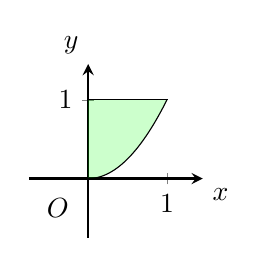
\begin{tikzpicture}
    \begin{axis}[standard,
            xtick={1},
            ytick={1},
            samples=1000,
            xlabel={$x$},
            ylabel={$y$},
            xmin=-0.5,xmax=1.2,
            ymin=-0.5,ymax=1.2,
            x=1cm,
            y=1cm/1,
           ]
\node[anchor=center,label=south west:$O$] at (axis cs:0,0){};
\addplot[name path=F,domain={0:1}]{x^2};
\addplot[name path=G, domain={0:1}]{1};
\addplot[fill=green, fill opacity=0.2] fill between [of=F and G, soft clip={domain=0:1}];
    \end{axis}
    \end{tikzpicture}
}
\end{center}
If we rewrite our region to be in terms of $y$, our function $y=x^2$ becomes $x=\sqrt{y}$ (keep positive one only). All together, we get
\begin{align*}
    0\leq &y\leq 1\\
    0\leq &x\leq \sqrt{y}
\end{align*}
Now, let's solve our integral.
\begin{align*}
    \int_0^1 \int_0^1 \int_{x^2} ^1 12 xze^{zy^2}\,dy\,dx\,dz&=\int_0^1 \int_0^1\int_0^{\sqrt{y}}12xze^{zy^2}\,dx\,dy\,dz\\
    &=\int_0^1\int_0^1\lrb{6x^2 ze^{zy^2}}_0^{\sqrt{y}}\,dy\,dz\\
    &=\int_0^1\int_0^1 6yze^{zy^2}\,dy\,dz\\
    &=\int_0^1\lrb{3e^{zy^2}}_0^1\,dz\tag{you could also do a u-sub $u=y^2$}\\
    &=\int_0^1 3e^{z}- 3\,dz\\
    &=\lrb{3e^z-3z}_0^1\\
    &=\lrp{3e-3}-\lrp{3-0}\\
    &=\boxed{3e-6}
\end{align*}
\textbf{(h)} $\displaystyle \int_0^2\int_0^{4-x^2}\int_0^x \frac{\sin 2z}{4-z}\,dy\,dz\,dx$

\Solution
\begin{align*}
    \int_0^2\int_0^{4-x^2}\int_0^x \frac{\sin 2z}{4-z}\,dy\,dz\,dx&=\int_0^2 \int_0^{4-x^2}\lrb{\frac{\sin 2z}{4-z}y}_0^x\,dz\,dx\\
    &=\int_0^2\int_0^{4-x^2}\frac{x\sin 2z}{4-z}\,dz\,dx
\end{align*}
This looks painful to solve in this order of integration, so let's change the order of integration to be $dx\,dz$ instead.

Notice that the region for $x,z$ is $0\leq x\leq2$ and $0\leq z\leq 4-x^2$.

Graphically, this looks like
\begin{center}
\resizebox{3.5cm}{!}{
    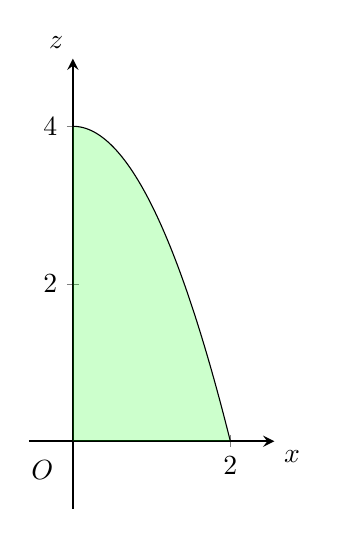
\begin{tikzpicture}
    \begin{axis}[standard,
            xtick={2},
            ytick={2,4},
            samples=1000,
            xlabel={$x$},
            ylabel={$z$},
            xmin=-0.2,xmax=2.2,
            ymin=-0.2,ymax=4.2,
            x=1cm,
            y=1cm/1,
           ]
\node[anchor=center,label=south west:$O$] at (axis cs:0,0){};
\addplot[name path=F,domain={0:2}]{4-x^2};
\addplot[name path=G, domain={0:2}]{0};
\addplot[fill=green, fill opacity=0.2] fill between [of=F and G, soft clip={domain=0:2}];
    \end{axis}
    \end{tikzpicture}
}
\end{center}
If we rewrite our region to be in terms of $z$, our function $z=4-x^2$ becomes $x=\sqrt{4-z}$ (keep positive one only).

All together, we get
\begin{align*}
    0\leq &z \leq 4\\
    0\leq &x \leq \sqrt{4-z}
\end{align*}
Now, let's solve our integral.
\begin{align*}
    \int_0^2\int_0^{4-x^2}\frac{x\sin 2z}{4-z}\,dz\,dx&=\int_0^4\int_0^{\sqrt{4-z}}\frac{x\sin 2z}{4-z}\,dx\,dz\\
    &=\int_0^4\lrb{\lrp{\frac{\sin 2z}{4-z}}\frac{1}{2}x^2}_0^{\sqrt{4-z}}\,dz\\
    &=\int_0^4\lrp{\frac{\sin 2z}{4-z}\frac{1}{2}\lrp{4-z}}\,dz\\
    &=\frac{1}{2}\int_0^4\sin 2z\,dz\\
    &=\frac{1}{2}\lrb{-\frac{1}{2}\cos 2z}_0^4\\
    &=\frac{1}{2}\lrp{-\frac{1}{2}\cos 8 +\frac{1}{2}}\\
    &=\boxed{\frac{-\cos 8+1}{4}}
\end{align*}
\textbf{Problem 4}

Find the volume of the region in the first octant bounded by the coordinate planes...

\textbf{(a)} ... the plane $y+z=2$, and the cylinder $x=4-y^2$

\Solution

Let's draw this from a front view and a top view. 

For the front view, we know that our $z$ is bounded below by $z=0$ since we're in the first octant. The plane $y+z=2$ bounds us from above.

For the top view, let's look at what happens at $z=0$. When $z=0$, $y+0=2\implies y=2$ and $x=4-y^2$. Don't forget that we're in the first octant, so $x,y\geq 0$.
\begin{figure}[h]
\centering
\begin{minipage}{.5\textwidth}
  \centering
  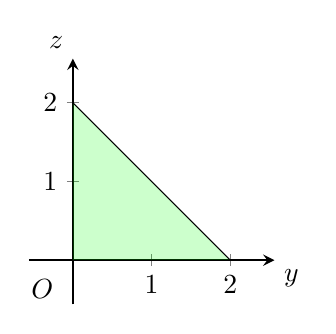
\begin{tikzpicture}
    \begin{axis}[standard,
            xtick={1,2},
            ytick={1,2},
            samples=1000,
            xlabel={$y$},
            ylabel={$z$},
            xmin=-0.2,xmax=2.2,
            ymin=-.2,ymax=2.2,
            x=1cm,
            y=1cm/1,
           ]
\node[anchor=center,label=south west:$O$] at (axis cs:0,0){};
\addplot[name path=F,domain={0:2}]{2-x};
\addplot[name path=G,domain={0:2}]{0};
\addplot[fill=green, fill opacity=0.2] fill between [of=F and G, soft clip={domain=0:2}];
    \end{axis}
    \end{tikzpicture}
  \caption*{front view}
  \label{fig:test1}
\end{minipage}%
\begin{minipage}{.5\textwidth}
  \centering
  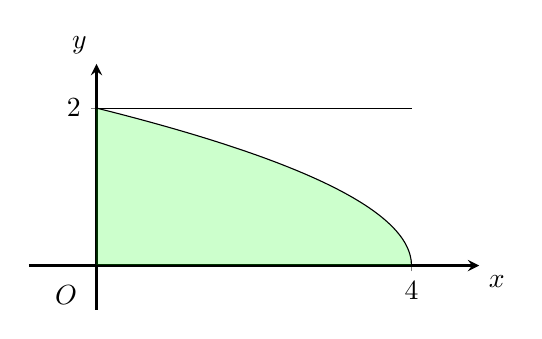
\begin{tikzpicture}
    \begin{axis}[standard,
            xtick={4},
            ytick={2},
            samples=1000,
            xlabel={$x$},
            ylabel={$y$},
            xmin=-0.2,xmax=4.2,
            ymin=-.2,ymax=2.2,
            x=1cm,
            y=1cm/1,
           ]
\node[anchor=center,label=south west:$O$] at (axis cs:0,0){};
\addplot[name path=F,domain={0:4}]{sqrt(4-x)};
\addplot[name path=G,domain={0:4}]{2};
\addplot[name path=H, domain={0:4}]{0};
\addplot[fill=green, fill opacity=0.2] fill between [of=F and H, soft clip={domain=0:4}];
    \end{axis}
    \end{tikzpicture}
  \caption*{top view}
  \label{fig:test2}
\end{minipage}
\end{figure}

All together, our region is
\begin{align*}
    0\leq &z \leq 2- y\\
    0\leq &y \leq \sqrt{4-x}\tag{$x=4-y^2\implies y^2=4-x$}\\
    0\leq & x \leq 4
\end{align*}
Our integral for the volume is
\begin{align*}
    V&=\int_0^4\int_0^{\sqrt{4-x}}\int_0^{2-y}\,dz\,dy\,dx\\
    &=\int_0^4\int_0^{\sqrt{4-x}}\lrb{z}_0^{2-y}\,dy\,dx\\
    &=\int_0^4\int_0^{\sqrt{4-x}} 2-y\,dy\,dx\\
    &=\int_0^4\lrb{2y-\frac{1}{2}y^2}_0^{\sqrt{4-x}}\,dx\\
    &=\int_0^4 2\sqrt{4-x}-\frac{1}{2}(4-x)\,dx\\
    &=\lrb{-\frac{4}{3}(4-x)^{3/2}+\frac{1}{4}(4-x)^2}_0^4\\
    &=-\lrp{-\frac{4}{3}(4)^{3/2}+\frac{1}{4}(4)^2}\\
    &=\frac{4}{3}(8)-4\\
    &=\boxed{\frac{20}{3}}
\end{align*}
\textbf{(b)} ... the plane $y=1-x$, and the surface $\displaystyle z=\cos \frac{\pi x}{2}$, $0\leq x \leq 1$.

\Solution

Let's draw this from a front view and a top view.

For the front view, we know that our $z$ is bounded below by $z=0$ since we're in the first octant. The plane $\displaystyle z=\cos\frac{\pi x}{2}$ bounds us from above.

For the top view, let's look at what happens at $z=0$. When $z=0$, $0=\cos\dfrac{\pi x}{2}\implies x=1$ and $y=1-x$. Don't forget that we're in the first octant, so $x,y\geq 0$.
\begin{figure}[h]
\centering
\begin{minipage}{.5\textwidth}
  \centering
  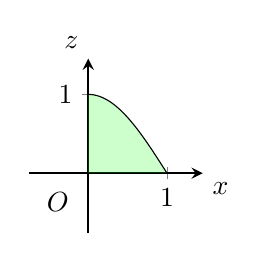
\begin{tikzpicture}
    \begin{axis}[standard,
            xtick={1},
            ytick={1},
            samples=1000,
            xlabel={$x$},
            ylabel={$z$},
            xmin=-0.5,xmax=1.2,
            ymin=-.5,ymax=1.2,
            x=1cm,
            y=1cm/1,
           ]
\node[anchor=center,label=south west:$O$] at (axis cs:0,0){};
\addplot[name path=F,domain={0:1}]{cos(3.14 159 * x / 2)};
\addplot[name path=G,domain={0:1}]{0};
\addplot[fill=green, fill opacity=0.2] fill between [of=F and G, soft clip={domain=0:1}];
    \end{axis}
    \end{tikzpicture}
  \caption*{front view}
  \label{fig:test2}
\end{minipage}%
\begin{minipage}{.5\textwidth}
  \centering
  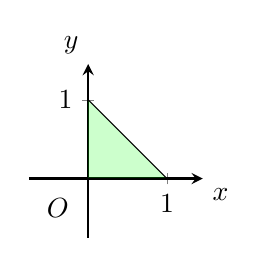
\begin{tikzpicture}
    \begin{axis}[standard,
            xtick={1},
            ytick={1},
            samples=1000,
            xlabel={$x$},
            ylabel={$y$},
            xmin=-0.5,xmax=1.2,
            ymin=-.5,ymax=1.2,
            x=1cm,
            y=1cm/1,
           ]
\node[anchor=center,label=south west:$O$] at (axis cs:0,0){};
\addplot[name path=F,domain={0:1}]{1-x};
\addplot[name path=G,domain={0:1}]{0};
\addplot[fill=green, fill opacity=0.2] fill between [of=F and G, soft clip={domain=0:1}];
    \end{axis}
    \end{tikzpicture}
  \caption*{top view}
  \label{fig:test2}
\end{minipage}
\end{figure}

All together, our region is
\begin{align*}
    0\leq &z \leq \cos \frac{\pi x}{2}\\
    0\leq &y \leq 1-x\\
    0\leq & x \leq 1
\end{align*}
Our integral for the volume is
\begin{align*}
    V&=\int_0^1\int_0^{1-x}\int_0^{\cos\frac{\pi x}{2}}\,dz\,dy\,dx\\
    &= \int_0^1\int_0^{1-x}\lrb{z}_0^{\cos\frac{\pi x}{2}}\,dy\,dx\\
    &= \int_0^1 \int_0^{1-x}\cos\frac{\pi x}{2}\,dy\, dx\\
    &=\int_0^1\lrb{\lrp{\cos \frac{\pi x}{2}}y}_0^{1-x}\,dx\\
    &=\int_0^1 \lrp{\cos \frac{\pi x}{2}}\lrp{1-x}\,dx\\
    &=\int_0^1\cos\frac{\pi x}{2}-\int_0^1 x\cos \frac{\pi x}{2}\,dx\\
    &u=x\hspace{2em}dv=\cos\frac{\pi x}{2}\,dx\\
    &du=dx\hspace{2em}v=\frac{2}{\pi}\sin\frac{\pi x}{2}\\
    &=\lrb{\frac{2}{\pi}\sin\frac{\pi x}{2}}_0^1 -\lrp{\lrb{\frac{2x}{\pi}\sin\frac{\pi x}{2}}_0^1-\frac{2}{\pi}\int_0^1 \sin \frac{\pi x}{2}\,dx}\\
    &=\lrp{\frac{2}{\pi}}-\lrp{\frac{2}{\pi}-\frac{2}{\pi}\lrb{-\frac{2}{\pi}\cos\frac{\pi x}{2}}_0^1}\\
    &=\frac{2}{\pi}-\lrp{\frac{2}{\pi}-\frac{2}{\pi}\lrp{\frac{2}{\pi}}}\\
    &=\boxed{\frac{4}{\pi^2}}
\end{align*}
\textbf{(c)} ... the plane $x+y=4$, and the cylinder $y^2+4z^2=16$.

\Solution

Let's draw this from a front view and a top view.

For the front view, we know that our $z$ is bounded below by $z=0$ since we're in the first octant. The cylinder $y^2+4z^2=16$ bounds us from above.

For the top view, let's look at  what happens at $z=0$. When $z=0$, $y^2+0=16\implies y=4$ (first octant only!) and $x+y=4$. Don't forget that we're in the first octant, so $x,y\geq 0$.
\begin{figure}[h]
\centering
\begin{minipage}{.5\textwidth}
  \centering
  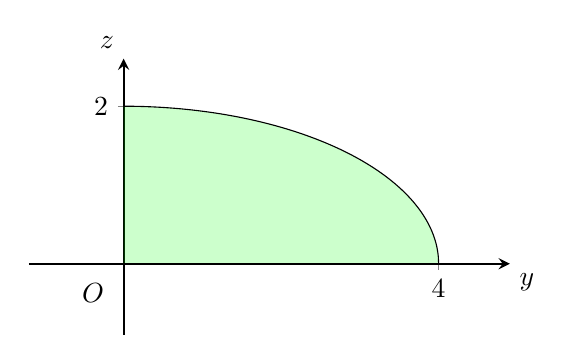
\begin{tikzpicture}
    \begin{axis}[standard,
            xtick={4},
            ytick={2},
            samples=1000,
            xlabel={$y$},
            ylabel={$z$},
            xmin=-0.5,xmax=4.2,
            ymin=-.5,ymax=2.2,
            x=1cm,
            y=1cm/1,
           ]
\node[anchor=center,label=south west:$O$] at (axis cs:0,0){};
\addplot[name path=F,domain={0:4}]{sqrt(4-0.25*x^2)};
\addplot[name path=G,domain={0:4}]{0};
\addplot[fill=green, fill opacity=0.2] fill between [of=F and G, soft clip={domain=0:4}];
    \end{axis}
    \end{tikzpicture}
  \caption*{front view}
  \label{fig:test2}
\end{minipage}%
\begin{minipage}{.5\textwidth}
  \centering
  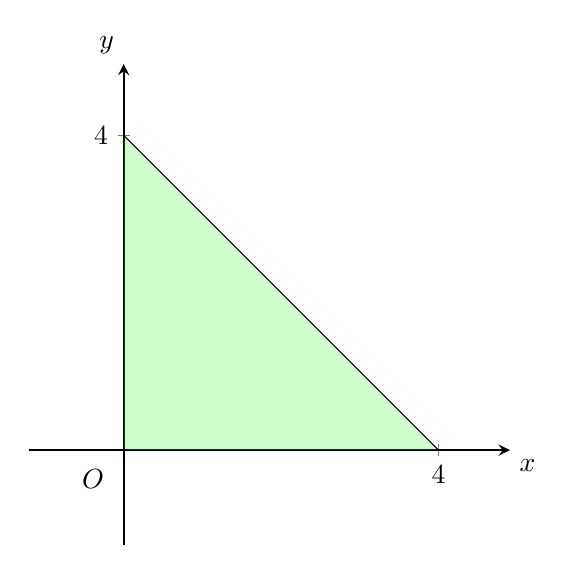
\begin{tikzpicture}
    \begin{axis}[standard,
            xtick={4},
            ytick={4},
            samples=1000,
            xlabel={$x$},
            ylabel={$y$},
            xmin=-0.5,xmax=4.2,
            ymin=-.5,ymax=4.2,
            x=1cm,
            y=1cm/1,
           ]
\node[anchor=center,label=south west:$O$] at (axis cs:0,0){};
\addplot[name path=F,domain={0:4}]{4-x};
\addplot[name path=G,domain={0:4}]{0};
\addplot[fill=green, fill opacity=0.2] fill between [of=F and G, soft clip={domain=0:4}];
    \end{axis}
    \end{tikzpicture}
  \caption*{top view}
  \label{fig:test2}
\end{minipage}
\end{figure}
All together, our region is
\begin{align*}
    0\leq &z\leq \sqrt{4-\frac{1}{4}y^2}\\
    0\leq &x \leq 4-y\\
    0\leq &y\leq 4
\end{align*}
There's a reason why we're not doing the $dz\,dy\,dx$ order. It results in a difficult, but not impossible to solve, integral.

Our integral for the volume is
\begin{align*}
    V&=\int_0^4\int_0^{\sqrt{4-\frac{1}{4}y^2}}\int_0^{4-y}\,dx\,dz\,dy\\
    &=\int_0^4\int_0^{\sqrt{4-\frac{1}{4}y^2}}\lrb{x}_0^{4-y}\,dz\,dy\\
    &=\int_0^4\int_0^{\sqrt{4-\frac{1}{4}y^2}} 4-y\,dz\,dy\\
    &=\int_0^4 \lrb{(4-y)z}_0^{\sqrt{4-\frac{1}{4}y^2}}\,dy\\
    &=\int_0^4 (4-y)\sqrt{4-\frac{1}{4}y^2}\,dy\\
    &=\int_0^4(4-y)\sqrt{\frac{1}{4}\lrp{16-y^2}}\\
    &=\frac{1}{2}\int_0^4 (4-y)\sqrt{16-y^2}\,dy\\
    &=\frac{1}{2}\lrp{\int_0^4 4\sqrt{16-y^2}\,dy-\int_0^4 y\sqrt{16-y^2}\,dy}\\
    &=2\int_0^4\sqrt{16-y^2}\,dy-\frac{1}{2}\int_0^4 y\sqrt{16-y^2}\,dy\\
    &=2\lrp{\frac{1}{4}\pi(4)^2}-\frac{1}{2}\lrb{-\frac{1}{3}\lrp{16-y^2}^{\frac{3}{2}}}_0^4\\
    &=8\pi -\frac{1}{2}\lrp{\frac{1}{3}(16)^{\frac{3}{2}}}\\
    &=8\pi -\frac{1}{2}\lrp{\frac{1}{3}(64)}\\
    &=\boxed{8\pi-\frac{32}{3}}
\end{align*}

You could have done a trig substitution for the integral of $\displaystyle \int_0^4 \sqrt{16-y^2}\,dy$, or you could have just realized that this is the area of a quarter-circle with radius $4$ :)

\textbf{Problem 5}

Find the average value of the function $f(x,y,z)=x^2+y^2+z^2$ over the cube in the first octant bounded by the coordinate planes and the planes $x=1$, $y=1$, and $z=1$.

\Solution

The average value is going to be the triple integral divided by the region. In this case, a cube of length $1$.
\begin{align*}
    f(x,y,z)_{
    \text{avg}}&=\frac{1}{(1)(1)(1)}\int_0^1\int_0^1\int_0^1 x^2+y^2+z^2\,dz\,dy\,dx\\
    &=\int_0^1\int_0^1\lrb{x^2z+y^2z+\frac{1}{3}z^3}_0^1\,dy\,dx\\
    &=\int_0^1\int_0^1 x^2+y^2 +\frac{1}{3}\,dy\,dx\\
    &=\int_0^1\lrb{x^2y+\frac{1}{3}y^3+\frac{1}{3}y}_0^1\,dx\\
    &=\int_0^1 x^2 +\frac{1}{3}+\frac{1}{3}\,dx\\
    &=\lrb{\frac{1}{3}x^3+\frac{1}{3}x+\frac{1}{3}x}_0^1\\
    &=\frac{1}{3}+\frac{1}{3}+\frac{1}{3}\\
    &=\boxed{1}
\end{align*}
\textbf{Problem 6}

What domain $D$ maximizes the value of the integral $\displaystyle \iiint_D 1-x^2-y^2-z^2\,dV$?

\Solution

If we want to maximize the value of the integral, the inside part of the integral, $1-x^2-y^2-z^2$ must always be positive in our domain $D$. Therefore,
\begin{align*}
    0\leq 1-x^2&-y^2-z^2\\
   x^2 + y^2& + z^2 \leq 1
\end{align*}
Don't forget that the formula for a sphere is \begin{align*}
    x^2+y^2+z^2=a^2
\end{align*}
Therefore, our domain is going to be a filled in sphere of radius $1$ centered at the origin.
\end{document}